\documentclass{article} % For LaTeX2e
\usepackage{nips2015,times}
\usepackage{hyperref}
\usepackage{url}
\usepackage{graphicx}
\graphicspath{ {./assets/} }
\usepackage{biblatex}
\addbibresource{refs.bib}


\usepackage{float}
\usepackage[inline]{enumitem}
\usepackage{booktabs}
\usepackage{multirow}
\usepackage[center]{caption}
\usepackage{subcaption}

\title{CSE 546 Assignment 3 - Actor-Critic Algorithms}


\author{
   Sailesh Reddy \\
   Department of Computer Science\\
   University at Buffalo, SUNY\\
   Buffalo, NY 14260 \\
   \texttt{saileshr@buffalo.edu}
   \And
   Mohammed Nasheed Yasin \\
   Department of Linguistics\\
   University at Buffalo, SUNY\\
   Buffalo, NY 14260 \\
   \texttt{m44@buffalo.edu}
}

% The \author macro works with any number of authors. There are two commands
% used to separate the names and addresses of multiple authors: \And and \AND.
%
% Using \And between authors leaves it to \LaTeX{} to determine where to break
% the lines. Using \AND forces a linebreak at that point. So, if \LaTeX{}
% puts 3 of 4 authors names on the first line, and the last on the second
% line, try using \AND instead of \And before the third author name.

\newcommand{\fix}{\marginpar{FIX}}
\newcommand{\new}{\marginpar{NEW}}

\nipsfinalcopy

\begin{document}


\maketitle

\begin{abstract}
    This report presents our experiments on three environments, \verb|CartPole-v1|, \verb|LunarLander-v2| and \verb|InvertedPendulum-v4|. These environments were selected from the \verb|ClassicalControl|, \verb|Box2D| and \verb|MuJoCo| collections respectively in the Gymnasium library \cite{1606.01540}. We applied Q Actor-Critic Algorithm to solve these environments and conducted a case study on the outcomes.
\end{abstract}


\section{Q Actor-Critic Algorithm}

\subsection{Network Architecture}
The policy(actor) network takes the state as input and outputs probability distributions over the action space. In the case of discrete action space, the value function (critic) net again takes the state as input and outputs estimate the Q value for each action In continuous action space. In the case of continuous action space, however, the value function (critic) net takes the state-action pair as input and outputs the Q value for that particular state-action pair.

\begin{figure}[H]
    \begin{center}
        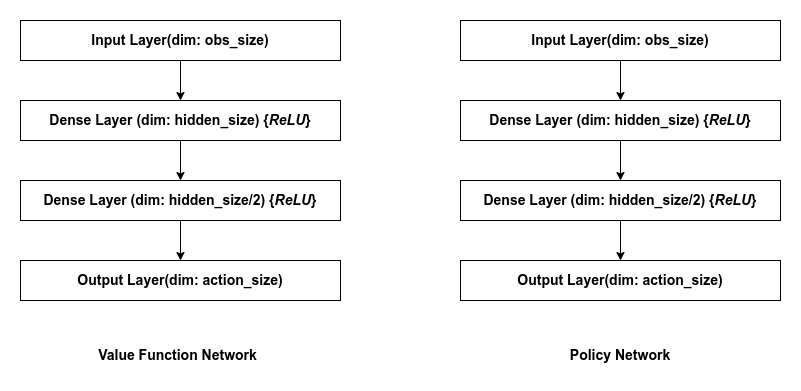
\includegraphics[width=\textwidth]{discrete.png}
    \end{center}
    \caption{Networks for Discrete Action Space}
\end{figure}

\begin{figure}[H]
    \begin{center}
        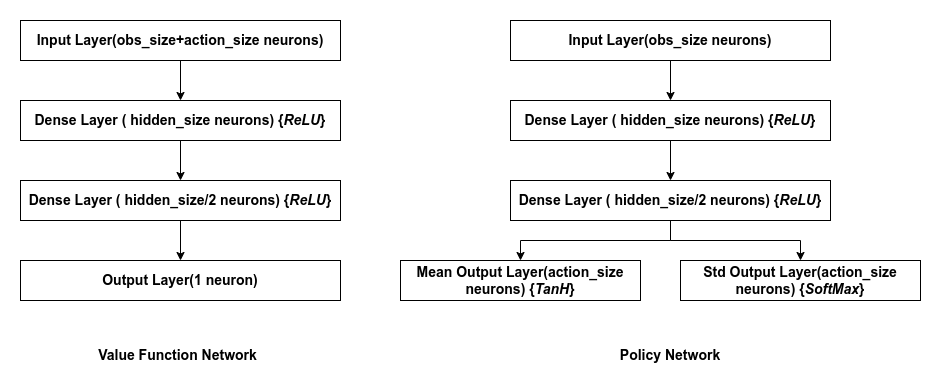
\includegraphics[width=\textwidth]{contionous.png}
    \end{center}
    \caption{Networks for Continuous Action Space}
\end{figure}

\subsection{Choosing Action}
The policy network takes the current state as input and outputs a probability distribution over actions. The agent chooses an action based on this distribution.

\subsection{Value Function update}
The value function network is updated using the Q-learning algorithm, which involves computing the TD error and updating the value estimates for the current state-action pair.

\subsection{Policy update}
The policy network is updated using the q value function, which involves computing the q value of the chosen action and updating the actor parameters to increase the probability of choosing that action in the future.

\section{Difference between Actor-Critic and Value-based approximation algorithms}

The main difference between the two approaches is that while value-based algorithms only learn the value function, actor-critic algorithms learn both a policy (actor) and an approximate estimate of the value function (critic) where the policy(actor) is updated based on the value function (critic).

\section{CartPole-v1}
\label{sec:cart-definition}

In the cart-pole problem version described by Barto, Sutton, and Anderson 
\cite{barto1983neuronlike} a pole is
connected to a cart through a joint that cannot be moved. The cart can move on a track
without any friction. The pole is positioned upright on the cart and the objective is to
keep the pole balanced by applying forces to the cart in either the left or right direction.
This environment has been visualized in Figure \ref{fig:cartpole-rendering}.

\begin{figure}[h]
    \begin{center}
        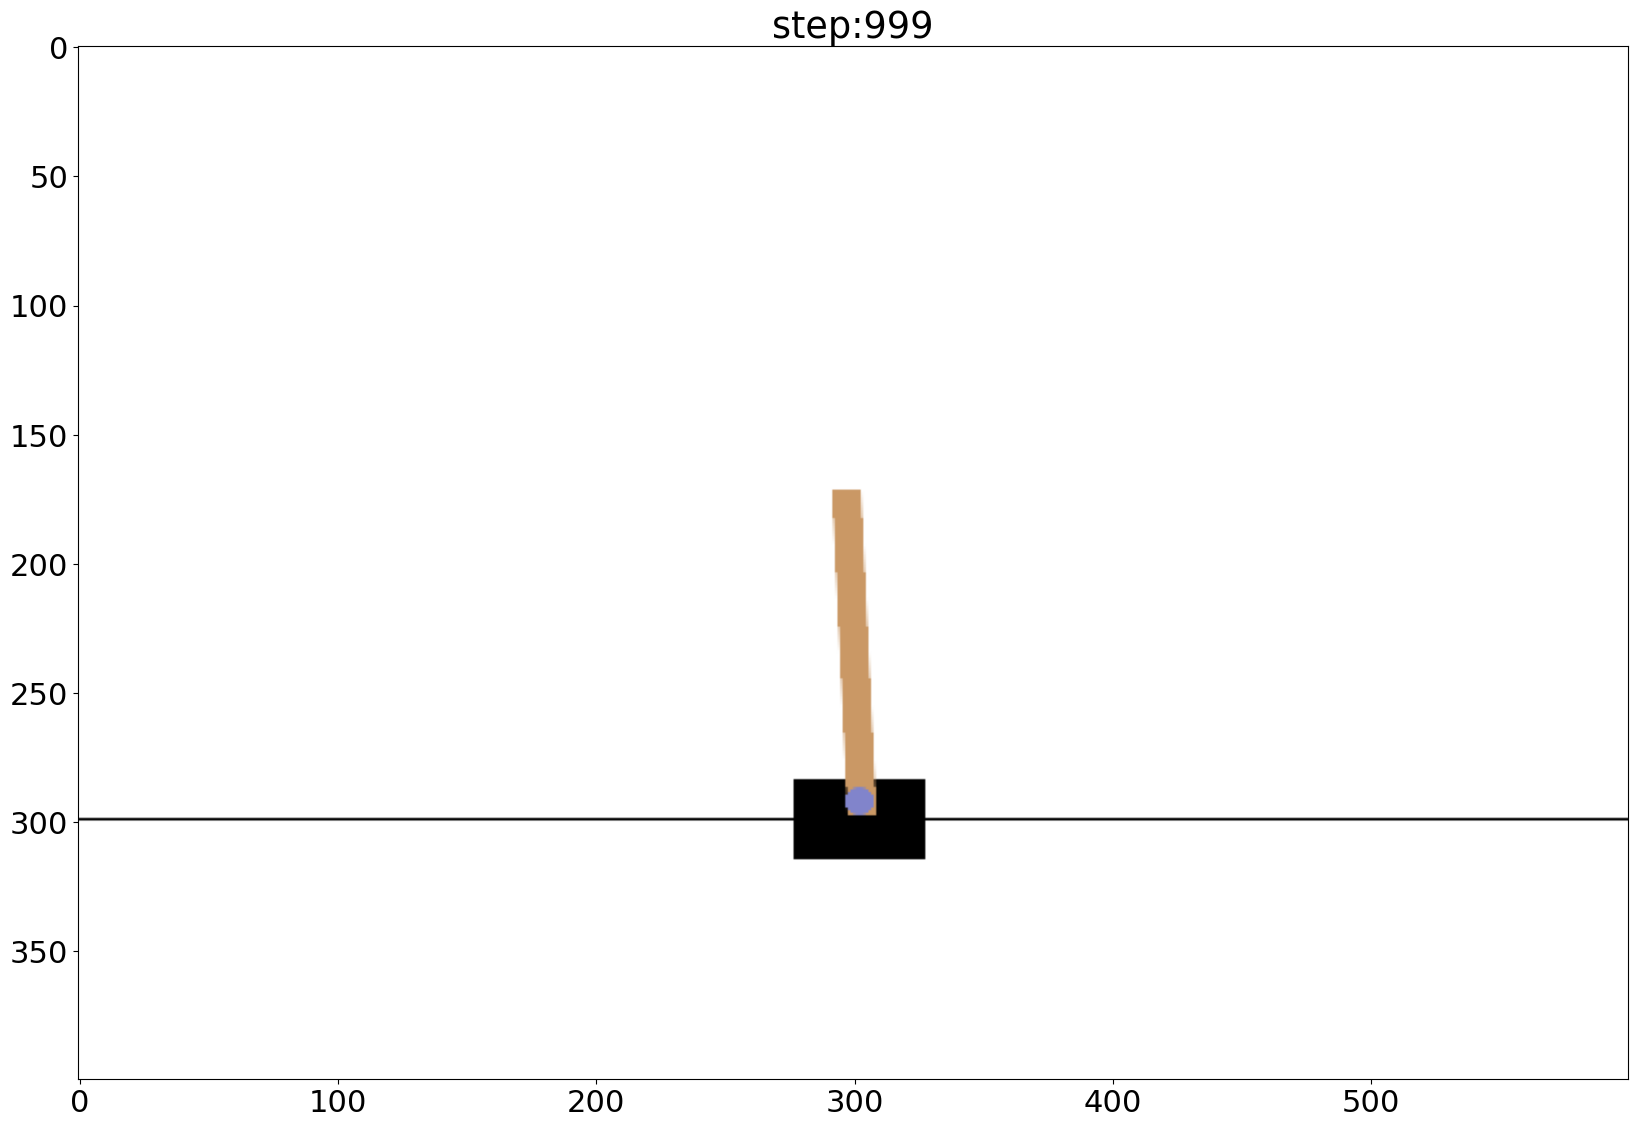
\includegraphics[width=\textwidth]{cartpole.png}
    \end{center}
    \caption{A frame from CartPole-v1}
    \label{fig:cartpole-rendering}
\end{figure}

\subsection{Action Space}
The action is an ndarray of shape (1,) that can take on values {0, 1} to indicate the
direction in which the cart is pushed with a fixed force.

\begin{itemize}
    \item 0: The cart is pushed to the left
    \item 1: The cart is pushed to the right
\end{itemize}

The velocity that is either decreased or increased by the force applied is not constant
and depends on the angle at which the pole is pointing. The center of gravity of the pole
affects the amount of energy required to move the cart beneath it.

\subsection{Observation Space}

The observation is an ndarray of shape (4,) where the values represent the positions and
velocities described next.

\begin{center}
    \begin{tabular}{cccc}
        \toprule
        Num & Observation & Min & Max \\
        \midrule
        0 & Cart Position & -4.8 & 4.8 \\
        1 & Cart Velocity & -Inf & Inf \\
        2 & Pole Angle & $\sim$ -0.418 rad (-24°) & $\sim$ 0.418 rad (24°) \\
        3 & Pole Angular Velocity & -Inf & Inf \\
        \bottomrule
    \end{tabular}
\end{center}

Although the ranges above indicate the possible values for each element in the observation
space, they do not reflect the allowed values of the state space in an ongoing episode.
Specifically:

\begin{itemize}
    \item The cart x-position (index 0) can be take values between \verb|(-4.8, 4.8)|,
    but the episode terminates if the cart leaves the \verb|(-2.4, 2.4)| range.
    \item The pole angle can be observed between \verb|(-.418, .418)| radians
    or \verb|(±24°)|, but the
    episode terminates if the pole angle is not in the range \verb|(-.2095, .2095)|
    or \verb|(±12°)|
\end{itemize}

\subsection{Rewards}

The objective of the task is to keep the pole upright for as long as possible. To encourage
this behavior, a reward of +1 is given for every step taken, including the final step when
the episode terminates. In version 1 of the task, the threshold for achieving a successful
outcome is set at 475.

\subsection{Start State}
All observations are assigned a uniformly random value in \verb|(-0.05, 0.05)|

\subsection{Episode End}
The episode terminates under these conditions:

\begin{enumerate}
    \item Termination: Pole Angle is greater than \verb|±12°|
    \item Termination: Cart Position is greater than \verb|±2.4| (center of the cart
    reaches the edge of the display)
    \item Truncation: Episode length is greater than \verb|500|
\end{enumerate}


\section{LunarLander-v2}

This environment represents a classic problem of optimizing rocket trajectory. Based on Pontryagin’s maximum principle, the optimal approach is to either fire the engine at full throttle or turn it off completely. As a result, this environment has discrete actions: the engine is either on or off.

Two versions of the environment are available: discrete and continuous. In our work we have used the discrete version. The landing pad is always located at coordinates \verb|(0,0)|, which are represented by the first two numbers in the state vector. It is possible to land outside of the landing pad. Since fuel is unlimited, an agent can learn to fly and land successfully on its first attempt.

\begin{figure}[h]
    \begin{center}
        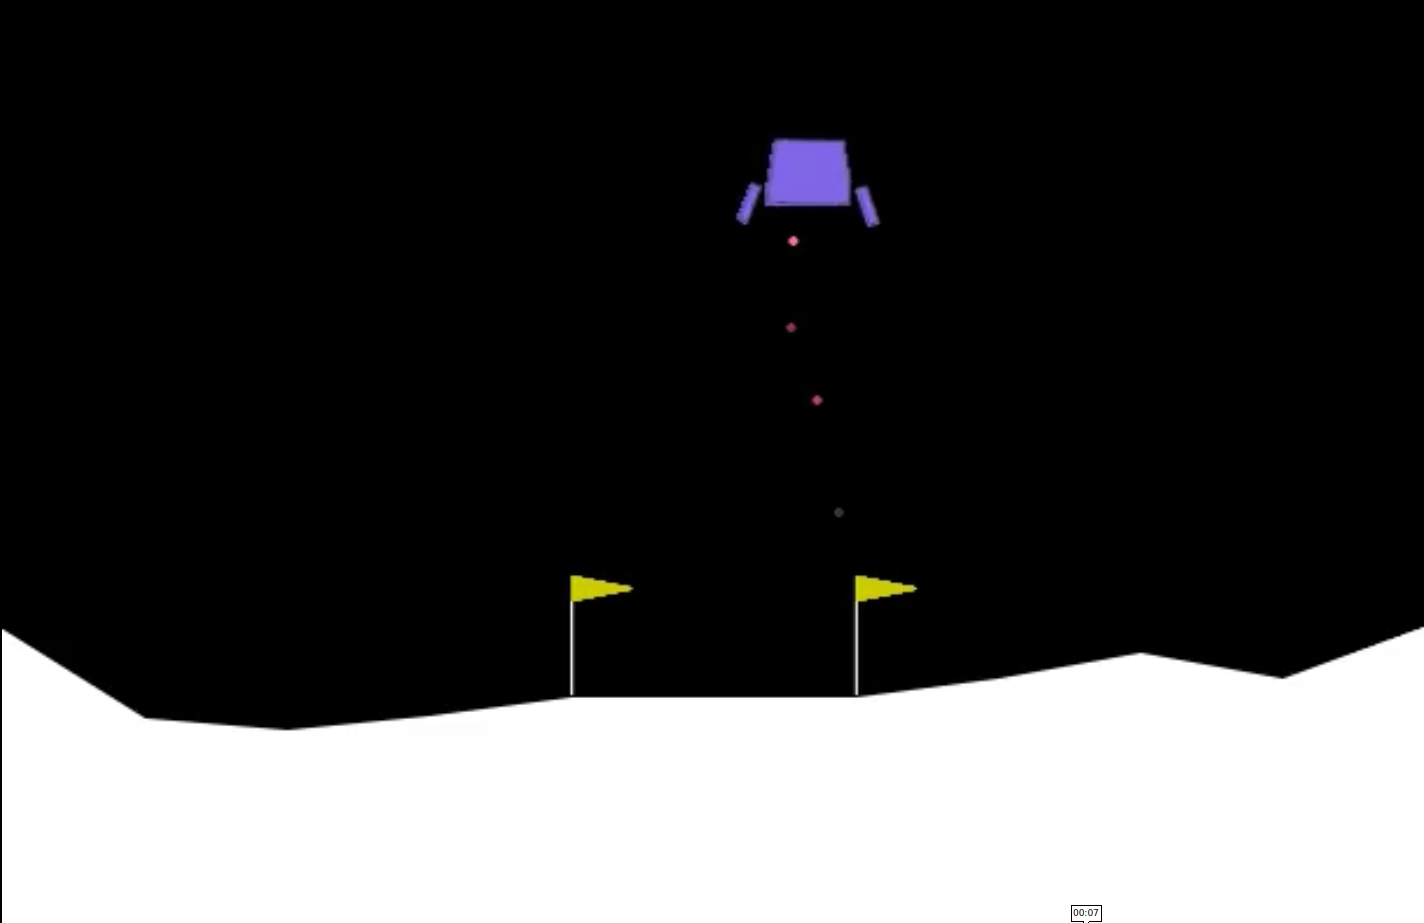
\includegraphics[width=\textwidth]{lunar_lander.png}
    \end{center}
    \caption{A frame from LunarLander-v2}
    \label{fig:mcar-rendering}
\end{figure}

\subsection{Observation Space}
The state of the environment is represented by an 8-dimensional vector that includes the \verb|x| and \verb|y| coordinates of the lander, its linear velocities in \verb|x| and \verb|y|, its angle and angular velocity, and two boolean values indicating whether each leg is in contact with the ground.

\subsection{Action Space}
Four discrete actions are available in this environment: remain idle, activate the left orientation engine, activate the main engine, or activate the right orientation engine.

\subsection{Reward}

A reward is given after each step in the environment. The total reward for an episode is calculated by summing the rewards for all steps within that episode. The reward for each step is determined by the following factors: \begin{itemize} \item The reward increases/decreases as the lander gets closer/further from the landing pad. \item The reward increases/decreases as the lander moves slower/faster. \item The reward decreases as the lander tilts more (angle not horizontal). \item The reward increases by 10 points for each leg in contact with the ground. \item The reward decreases by 0.03 points for each frame a side engine is firing. \item The reward decreases by 0.3 points for each frame the main engine is firing. \end{itemize} An additional reward of -100 or +100 points is given for crashing or landing safely, respectively. An episode is considered solved if it scores at least 200 points.

\subsection{Starting State}
At the beginning of each episode, the lander is positioned at the top center of the viewport and a random initial force is applied to its center of mass.


\subsection{Episode End}
An episode terminates if any of the following conditions are met: \begin{enumerate} \item The lander crashes (its body comes into contact with the moon). \item The lander moves outside of the viewport (its \verb|x| coordinate is greater than 1). \item The lander is not awake. According to the Box2D documentation, a body that is not awake does not move or collide with any other body. \end{enumerate}

\section{InvertedPendulum-v4}

This environment is the cart pole environment based on the work done by Barto, Sutton, and Anderson \cite{barto1983neuronlike}. This has a similar problem description to the classic environment but is powered by the Mujoco physics simulator - allowing for more complex experiments (such as varying the effects of gravity). This environment involves a cart that can move linearly, with a pole fixed on it at one end and another end free. The cart can be pushed left or right, and the goal is to balance the pole on the top by applying forces on the cart.

\begin{figure}[h]
    \begin{center}
        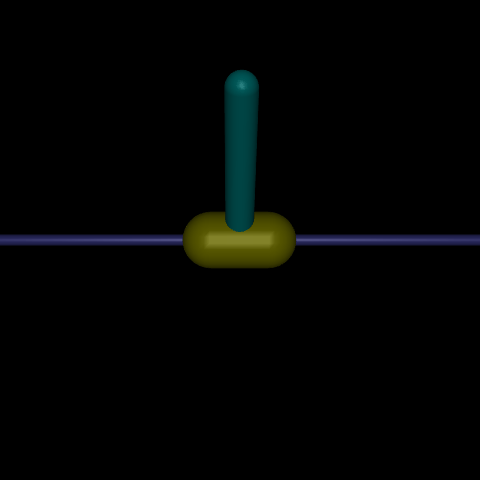
\includegraphics[width=\textwidth]{inverted_pendulum.png}
    \end{center}
    \caption{A frame from InvertedPendulum-v4}
    \label{fig:invpendulum-rendering}
\end{figure}

\subsection{Observation Space}
The state of the environment is represented by a 4-dimensional vector that includes the following.

\begin{center}
    \begin{tabular}{cccc}
        \toprule
        Num & Observation & Min & Max \\
        \midrule
        0 & Cart Position & -Inf & Inf \\
        1 & Pole Vertical Angle & -Inf & Inf \\
        2 & Cart Linear Velocity & -Inf & Inf \\
        3 & Pole Angular Velocity & -Inf & Inf \\
        \bottomrule
    \end{tabular}
\end{center}

\subsection{Action Space}
The agent takes a 1-dimensional vector for actions.

The action space is a continuous (action) in the range [-3, 3], where action represents the numerical force applied to the cart (with magnitude representing the amount of force and sign representing the direction)

\subsection{Reward}
The goal is to make the inverted pendulum stand upright (within a certain angle limit) as long as possible - as such a reward of +1 is awarded for each timestep that the pole is upright.

\subsection{Starting State}
All observations start in the state (0.0, 0.0, 0.0, 0.0) with a uniform noise in the range of [-0.01, 0.01] added to the values for stochasticity.

\subsection{Episode End}
The episode terminates when any of the following happens: \begin{enumerate}
\item The episode duration reaches 1000 timesteps.
\item Any of the state space values is no longer finite.
\item The absolute value of the vertical angle between the pole and the cart is greater than 0.2 radians.
\end{enumerate}

\section{Training and Evaluation Results}

\begin{figure}[H]
    \begin{center}
        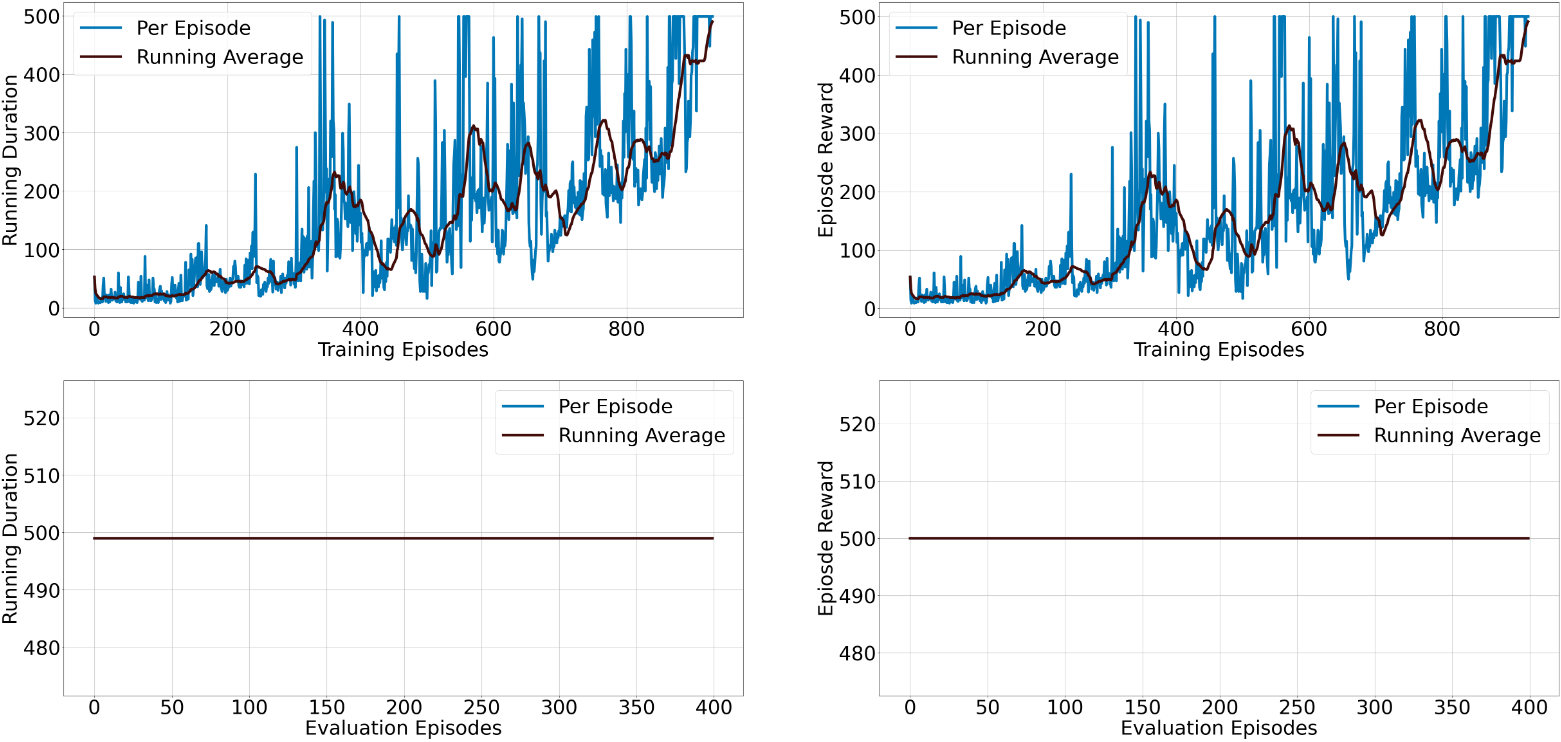
\includegraphics[width=\textwidth]{qac_cartpole.png}
    \end{center}
    \caption{Cart Pole Training and Evaluation}
\end{figure}

\begin{figure}[H]
    \begin{center}
        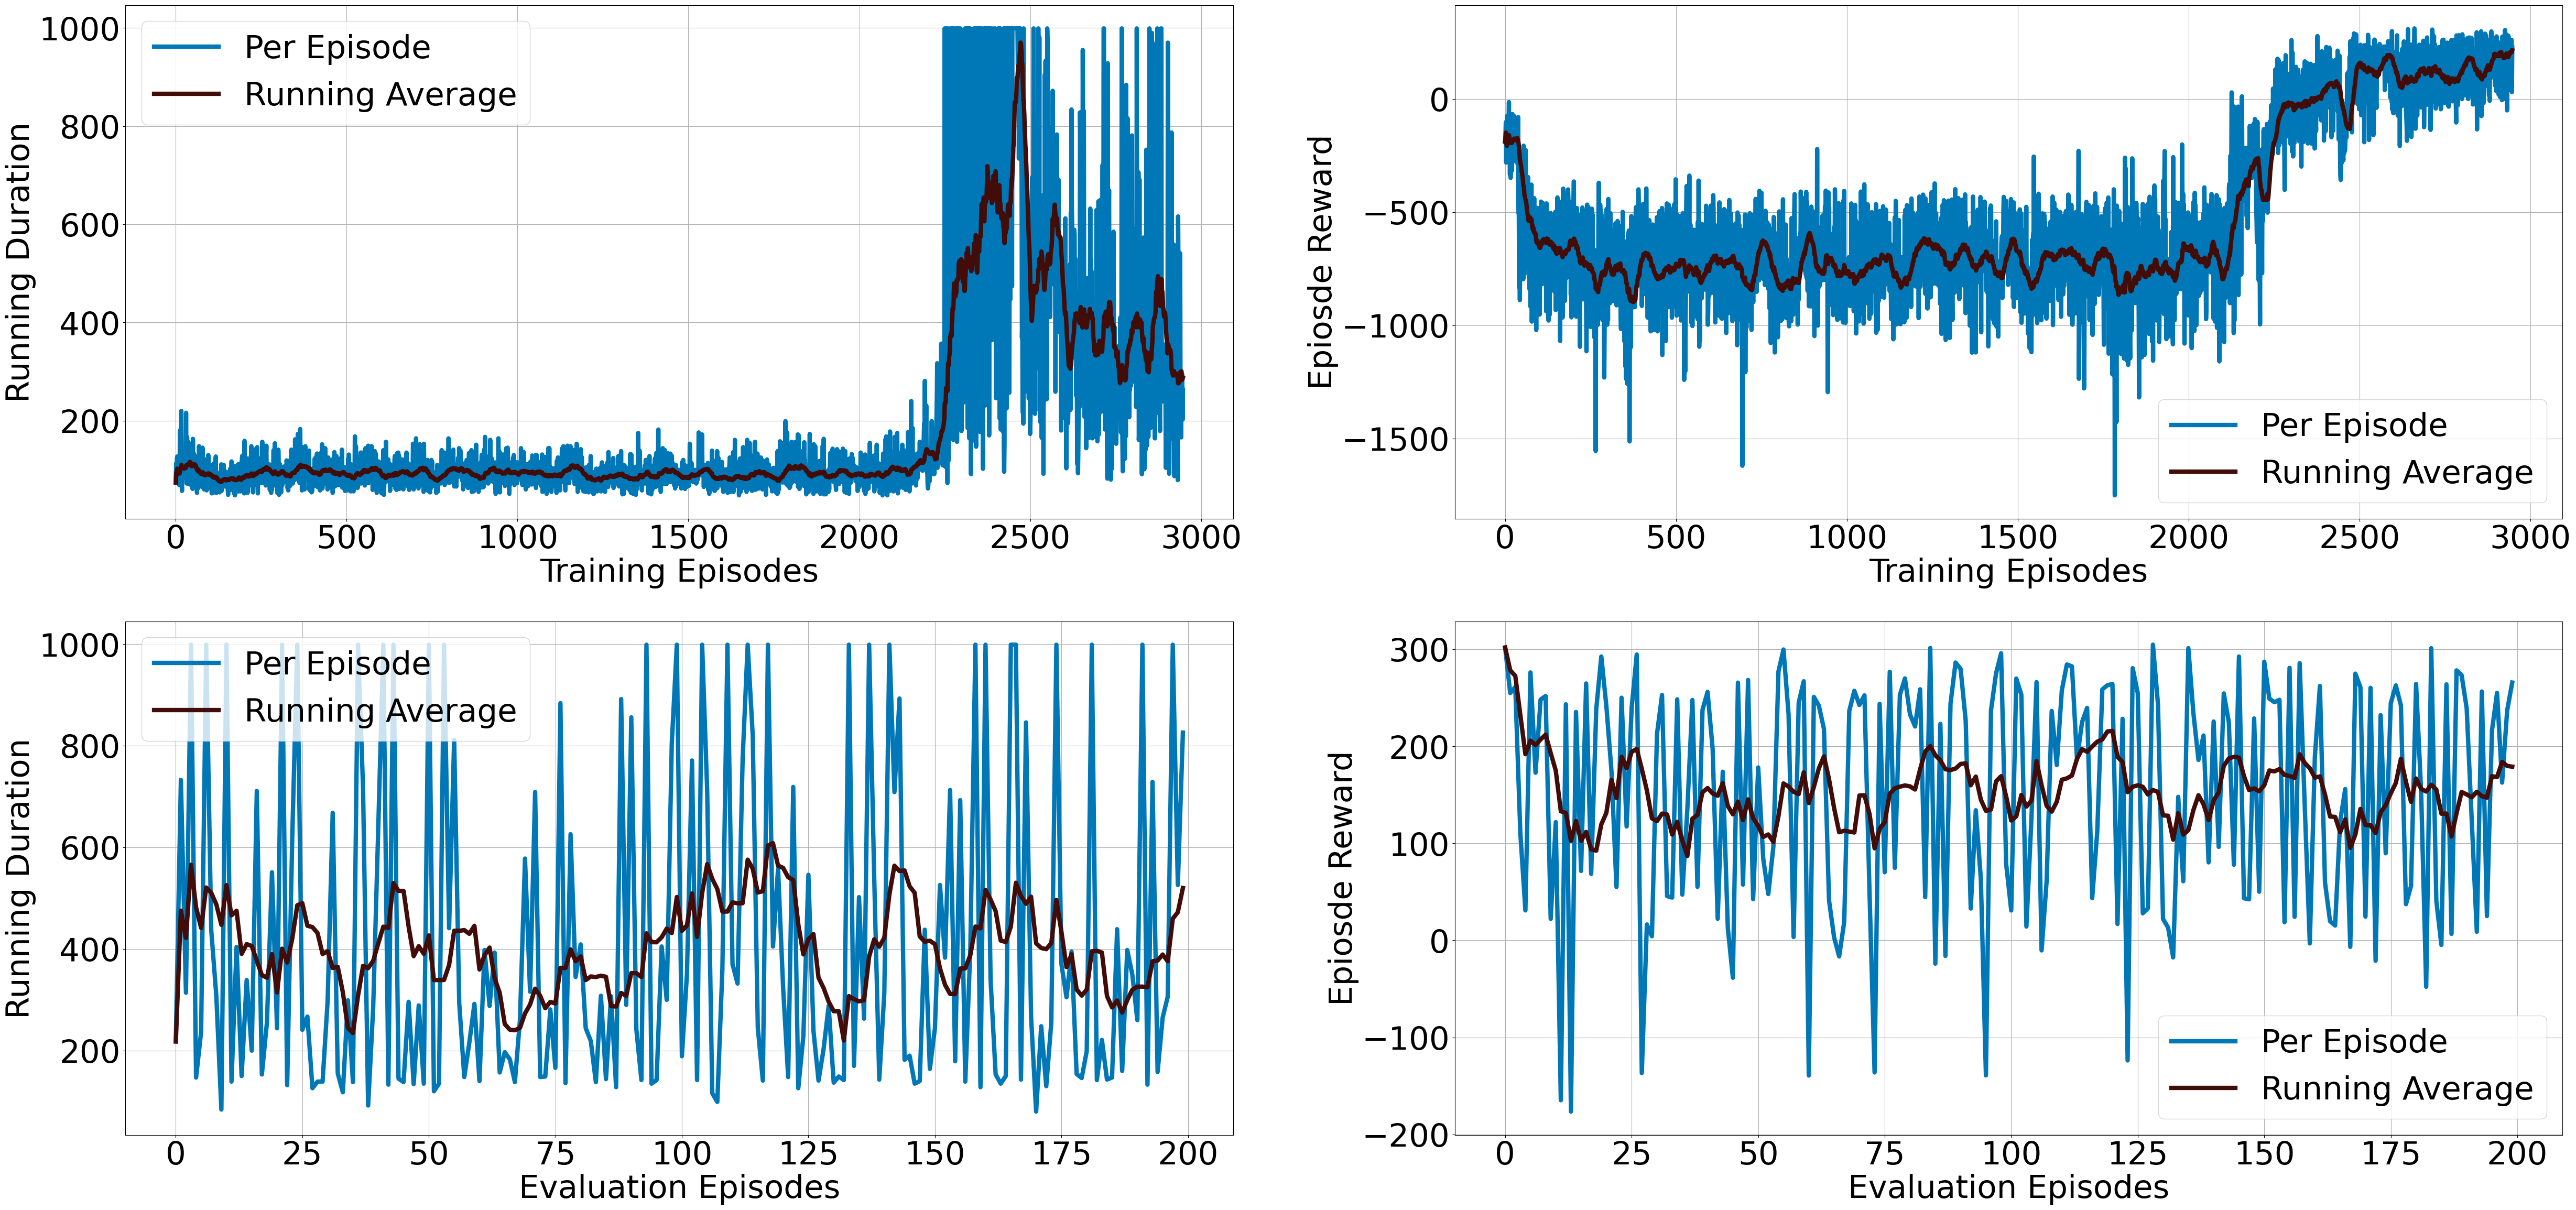
\includegraphics[width=\textwidth]{qac_lunar.png}
    \end{center}
    \caption{Lunar Lander Training and Evaluation}
\end{figure}

\begin{figure}[H]
    \begin{center}
        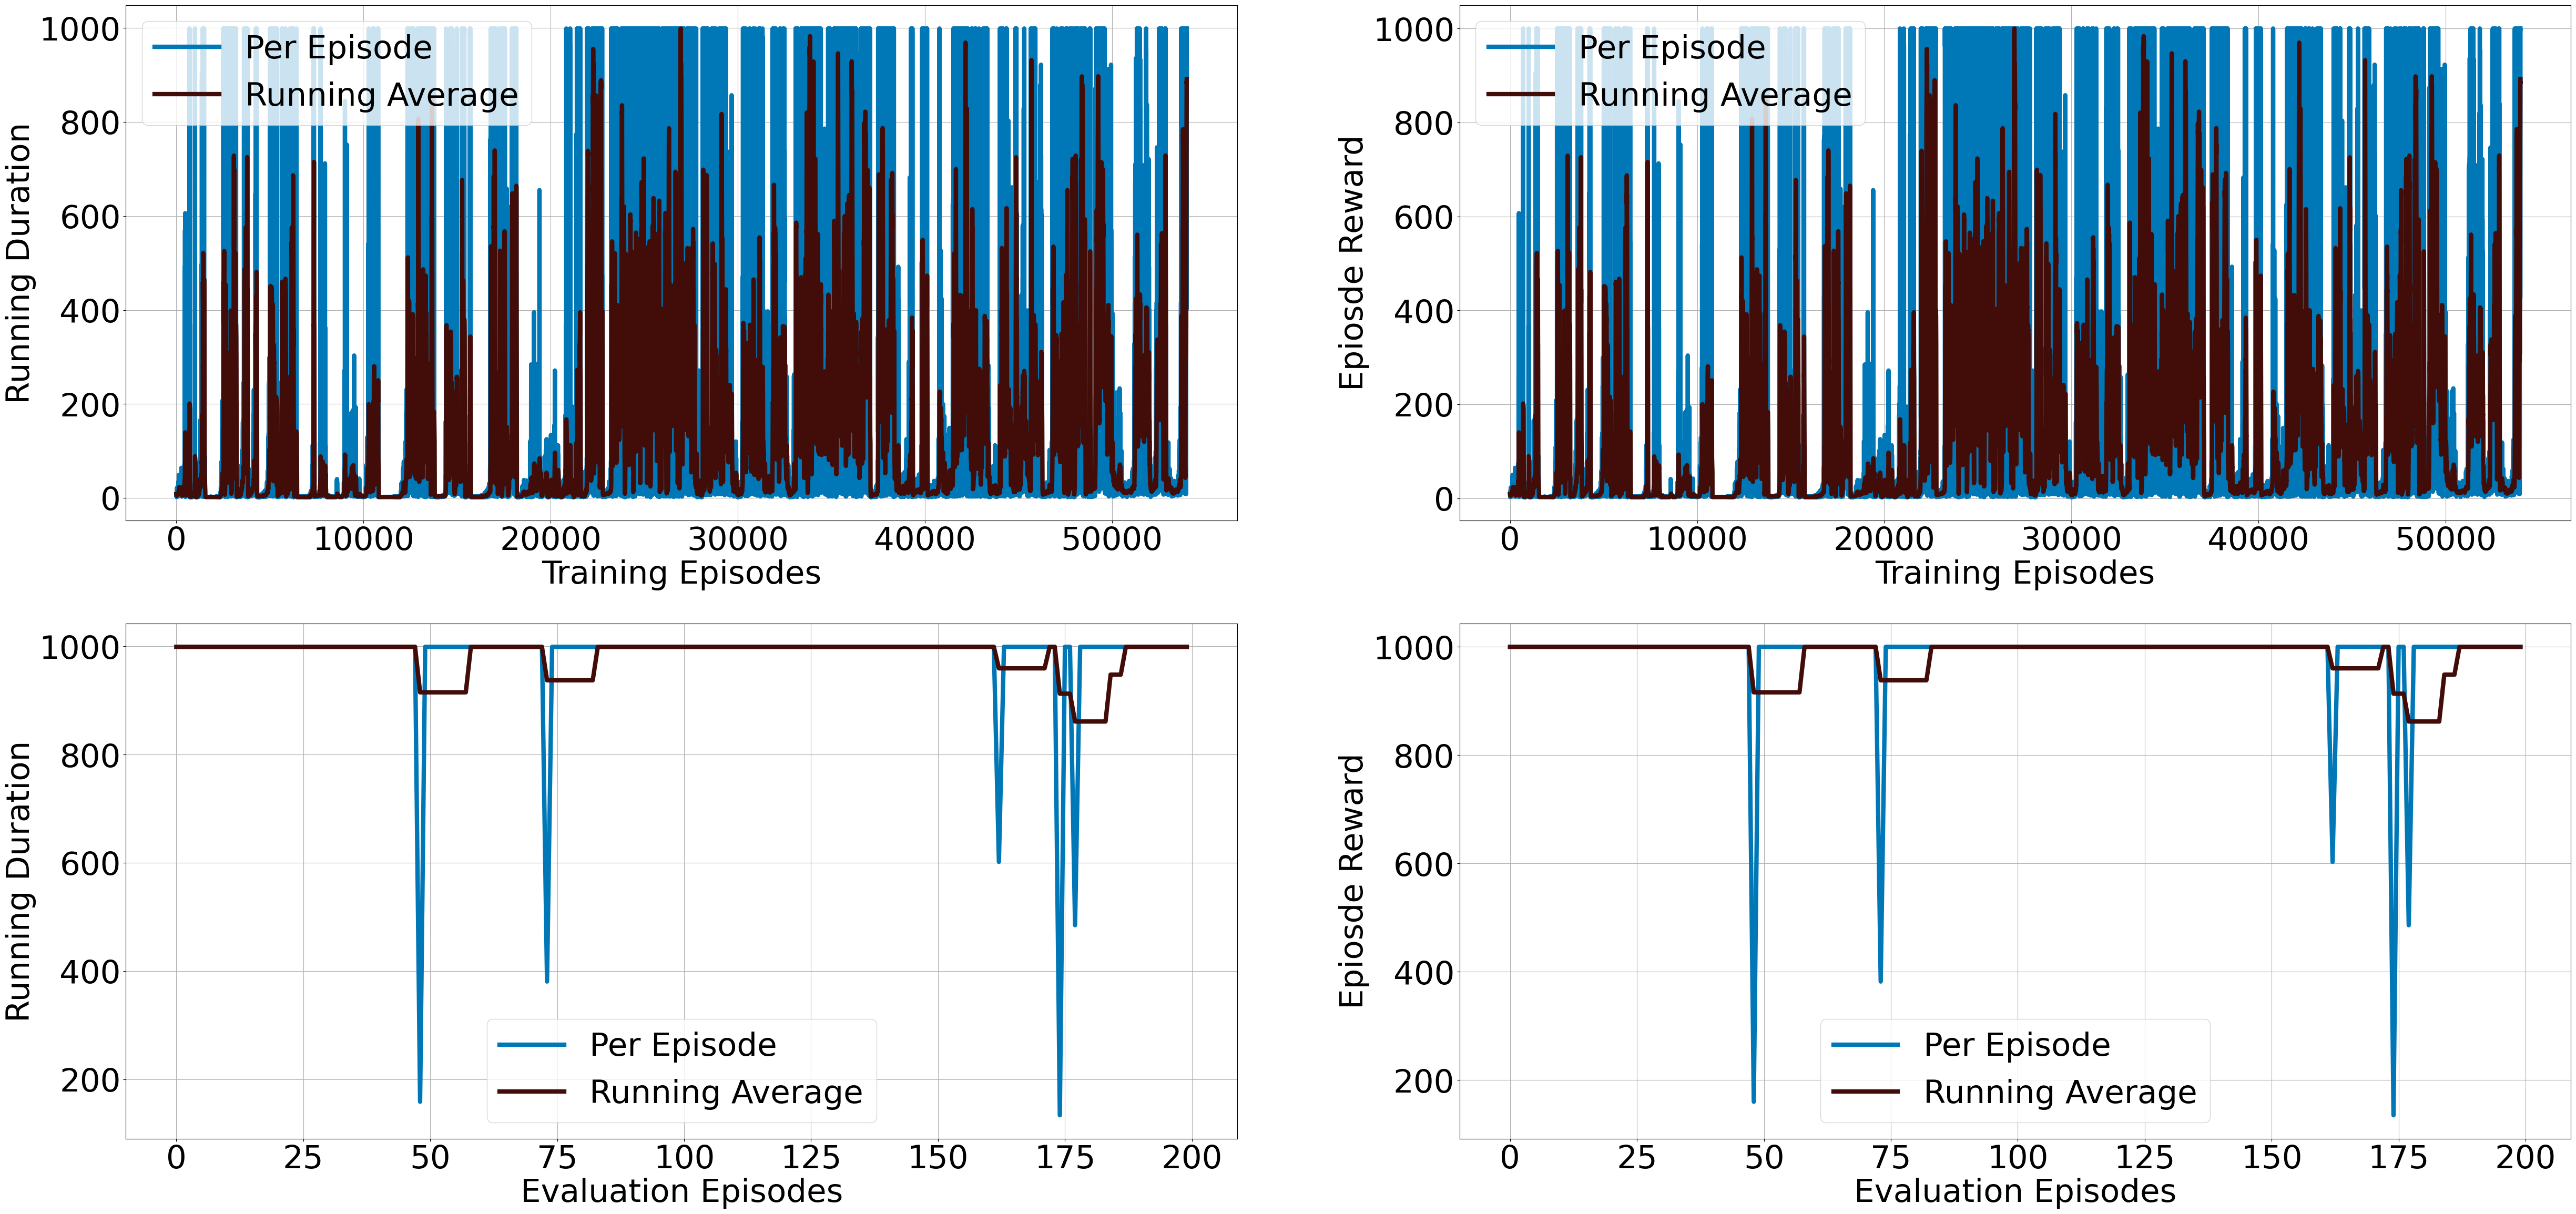
\includegraphics[width=\textwidth]{qac_invpendulum.png}
    \end{center}
    \caption{Inverted Pendulum Training and Evaluation}
\end{figure}

\printbibliography

\end{document}